\section{Метод многих сфер}

Метод многих сфер предназначен для аппроксимации электростатического взаимодействия между проводящими объектами произвольных форм.
Космический аппарат или космический мусор моделируется набором сфер с фиксированными размерами и относительными положениями (рис.\ref{ris:sp_msm}).
Внешняя сфера используется для разрешения сил и вращающих моментов на теле для определения оптимального решения параметров модели.
Предположим далее, что оптимальные относительные положения и размеры $n$ сфер в модели уже определены.
Получившийся набор сфер должен перемещаться и вращаться как изначальное тело.
Внешнюю сферу так же можно заменить другим объектом общей формы, описанным с помощью набора заряженных сфер.
Для каждого объекта нужно определить начало отсчета. Для аппарата на рисунке \ref{ris:sp_msm} это будет точка $O$. 

\begin{figure}[H]
	\center{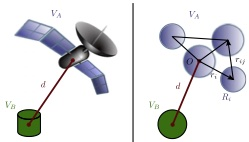
\includegraphics[scale=1.0]{spacecraft_msm.jpeg}}
	\caption{Концептуальное описание метода многих сфер}
	\label{ris:sp_msm}
\end{figure}

Абсолютное электростатическое напряжение предполагается расположенным на космическом аппарате.
При этом кулоновская сила взаимодействия между сферами зависит от заряда каждой сферы.
Напряжение $\Phi_i$ на каждой сфере зависит как от заряда самой сферы, так и от заряда соседних с ней сфер и определяется по формуле \ref{eq:voltage} \cite{2sph}.

\begin{equation}
\label{eq:voltage}
	\Phi_i = k_c \frac{q_i}{R_i} + \sum_{j=1,j\neq i}^{m} k_c \frac{q_j}{r_{i,j}},
\end{equation}
где $R_i$ – радиус $i$-ой сферы, $r_{i,j} = r_j - r_i$ – расстояние между центрами соседних сфер, $k_c = \frac{1}{4\pi\varepsilon_0} = 8.99 * 10^9 \frac{N*m^2}{C^2}$ – постоянная Кулона, $q_i$ – заряд $i$-ой сферы.

Линейные отношение каждой из $m = n + 1$ сфер ($n$ сфер описывают тело и одна внешняя) в системе можно представить в матричном виде (\ref{eq:voltage_matr}) \cite{msm}.

\begin{equation}
\label{eq:voltage_matr}
	\Phi = k_c [C_m]^{-1} q,
\end{equation}
где $\Phi = [\Phi_A, \Phi_A, \dots, \Phi_A, \Phi_B]^T$ – вектор напряжений, $q = [q_1, q_2, \dots, q_n, q_b]^T$ – вектор зарядов, $C_m$ – матрица ёмкостей, обратная матрица для которой записана в (\ref{eq:cm_inv}).
$V_A$ – напряжение каждой сферы тела, $V_B$ – напряжение внешней сферы.

\begin{equation}
\label{eq:cm_inv}
	[C_m]^{-1} = 
	\begin{pmatrix}
		\frac{1}{R_1}	&	\frac{1}{r_{1,2}}	&	\dots		&	\frac{1}{r_{1,n}}	&	\frac{1}{r_{1,B}} \\
		\frac{1}{r_{1,2}}	&	\frac{1}{R_1}	&	\dots		&	\vdots		&	\vdots \\
		\vdots		&	\ddots		&	\ddots	&	\vdots		&	\vdots \\
		\frac{1}{r_{n,1}}	&	\dots			&	\dots		&	\frac{1}{R_n}	&	\frac{1}{r_{n,B}} \\
		\frac{1}{r_{B,1}}	&	\dots			&	\dots		&	\frac{1}{r_{B,n}}	&	\frac{1}{R_B}
	\end{pmatrix},
\end{equation}
где $r_{i,B} = d - r_i$.

